% !TEX root = ../../mat701_notes.tex
\newpage

% bit on expanding real analysis. ultimate goal to integrate spaces of functions, along lines of functional analysis. ie use functions instead of real numbers.

% SKip chapters 1--2 of book & Being with chapter 3

\section{Lebesgue Outer Measure}


We want to assign a notion of `size' to sets. We denote this `size' by $\nu$. Let $\R^n= \{(x_1,\ldots,x_n) \colon x_i \in \R\}$ denote ordinary Euclidean space. By an `interval' in $\R^n$, we mean a set $\{ (a_1,b_1) \times (a_2,b_2) \times \cdots \times (a_n,b_n) \colon a_i,b_i \in \R^n, a_i<b_i\}$. By a closed interval in $\R^n$, we mean a set $\{ [a_1,b_1] \times [a_2,b_2] \times \cdots \times [a_n,b_n] \colon a_i,b_i \in \R^n, a_i<b_i\}$. We will often say `box', which will always mean an open or closed interval in $\R^n$. 
	\[
	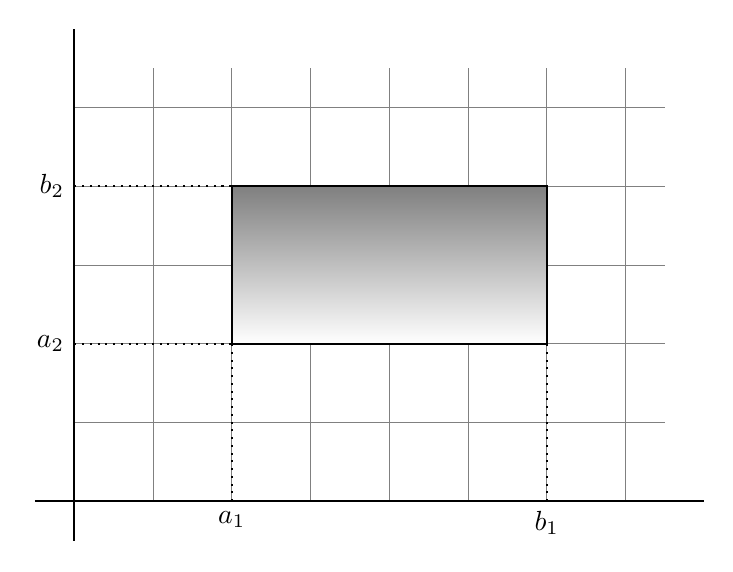
\begin{tikzpicture}[thick]
	\draw[gray,very thin] (0,0) grid (7.5,5.5);
	\draw (0,-0.5) -- (0,6);
	\draw (-0.5,0) -- (8,0);
	\shadedraw (2,2) -- (6,2) -- (6,4) -- (2,4) -- (2,2); % \draw[fill=gray!15]
	\draw[dotted] (2,0) -- (2,2);
	\draw[dotted] (6,0) -- (6,2);
	\draw[dotted] (0,2) -- (2,2);
	\draw[dotted] (0,4) -- (2,4);
	\node[below] at (2,0) {$a_1$};
	\node[below] at (6,0) {$b_1$};
	\node[left] at (0,2) {$a_2$};
	\node[left] at (0,4) {$b_2$};
	\end{tikzpicture}
	\]
In defining a `size' for sets, it makes sense to begin with a simple shape like a box. In the case of the plane, we know the a good notion of size is the area, and the area of a box $[a_1,b_1] \times [a_2,b_2]$ is $(b_1-a_1) \cdot (b_2-a_2)$. We can immediately generalize this to $\R^n$ as follows: if $I \subset \R^n$ is an interval, then we define
	\[
	\nu(I):= \prod_{j=1}^n (b_j - a_j)= (b_1-a_1)(b_2-a_2) \cdots (b_n-a_n)
	\]


\noindent But the question remains, how do we generalize this to an arbitrary region $E$? Given the above definition, it is natural to try to generalize to arbitrary sets $E$ by approximating $E$ by boxes, i.e. an open covering $\{I_k\}$ by intervals.

% Blob picture covered by boxes

It then becomes clear that whatever the measure of $E$ is, it should satisfy
	\[
	\nu(E) \leq \sum_k \nu(I_k),
	\]
since the intervals cover $E$. After all, it would be strange indeed to allow $E$ to have greater measure than its covering. Furthermore measure is going to be defined in terms of coverings, then the measure need be invariant of the choice of covering. These ideas are our guiding principles. So we take the following definition 

\begin{dfn}[Outer Measure]
For a set $E \subset \R^n$, the outer measure (or exterior measure) of $E$, denoted $\ext{E}$, is the function $\nu: \R^n \to [0,\infty)$ given by
	\[
	\ext{E}:= \inf_{E \subset \cup_k I_k} \sum \nu(I_k),
	\]
where the infimum is taken over all \emph{countable} coverings $\{I_k\}$ of $E$. 
\end{dfn}

The coining of `outer measure' is immediately obvious---we are measuring the size of a set via external objects, namely the open cover. However, less obvious is the need to restrict to countable coverings. The need to eliminate uncountable coverings is apparent as then trouble arises defining the summation. But why not only allow finite coverings? For this consider the case $E= \Q \cap [0,1]$. 

% insert dotted unit interval [0,1]
In any finite covering of $[0,1]$ by intervals, the intervals cannot all be pairwise disjoint. The reader will confirm, with a bit of thought, that if the intervals were all pairwise disjoint then there would be a rational number missed by the `covering.' But this contradicts the fact that the collection was an open cover. The the only possible open covering by intervals is the entire interval itself so that $\inf \sum \nu(I_k)=1$. This violates the notation that there isn't any `length' or `area' here since we have a sparse collection of points. Furthermore, the same logic applies to the set $E'=\Q^C \cap [0,1]$. So if the outer measure of $E$ were 1, then this would be true too of $E'$. But clearly the outer measure of $[0,1]$ is 1. Now $[0,1]=E \cup E'$, and $E \cap E'=\emptyset$. As $1+1 \neq 1$, this breaks countable subadditivity of the measure we are trying to define. By defining the outer measure in terms of countable covers, we obtain the expected answer $\ext{E}=0$. 

\begin{ex}
Let $E=\Q \cap [0,1]$ and $\ep>0$ be given. Since $\Q$ is countable, so too is $E$ countable. Enumerate the rationals in $E$ as $\{q_1,q_2,\ldots,q_n,\ldots\}$. Now the set $\{O_n\}_{n \in \N}$, where $O_n:= (q_n- \frac{1}{2^{n+k+1}}, q_n+\frac{1}{2^{n+k+1}})$ and $k \in \N$ is fixed, is a (countable) open covering of $E$ by intervals. Furthermore, the $O_n$ are pairwise disjoint. Choose $k$ sufficiently large so that $2^{-k}<\ep$. The measure of this covering is then
	\[
	\sum_{n=1}^\infty \nu(O_n)= \sum_{n=1}^\infty \left[ \left(q_n+\frac{1}{2^{n+k+1}}\right) - \left(q_n- \frac{1}{2^{n+k+1}}\right) \right]= \sum_{n=1}^\infty 2 \cdot \dfrac{1}{2^{n+k+1}}= \dfrac{1}{2^k} \sum_{n=1}^\infty \dfrac{1}{2^n}= \dfrac{1}{2^k}<\ep.
	\] \xqed
\end{ex}

As a final remark, observe that the exterior measure is a function to the nonnegative extended real line; that is, the exterior measure allows infinite values. Sets with an infinite exterior measure are considered measurable. For example, our intuition is that $\R$ should have infinite length and the reader routinely verifies that $\ext{\R}=\infty$. The outer measure $\ext{\cdot}$ defined above does meet all our guiding principles as the following proposition verifies. 

\begin{prop} \label{prop:outermprop} \hfill
	\begin{enumerate}[(i)]
	\item $\nu(\emptyset)=0$.
	\item Monotonicity: if $E_1 \subset E_2$, then $|E_1|_e \leq |E_2|_e$.
	\item Countable Subadditivity: $\displaystyle \ext{\bigcup_{k=1}^\infty E_k} \leq \sum_{k=1}^\infty |E_k|_e$
	\end{enumerate}
\end{prop}

\pf \\
\noindent$(i)$ This holds essentially by fiat. \\

\noindent$(ii)$ This follows immediately from the fact that we are taking an infimum and any open cover of $E_2$ is an open cover of $E_1$. \\

\noindent$(iii)$ Let $E:=\ext{\bigcup_{k=1}^\infty E_k}$. If any of the $E_k$ have infinite exterior measure, the result is immediate. Assume then that $\ext{E_k}<\infty$ for all $k$. Choose $\ep>0$ and cover each $E_k$ by intervals $\{I_n\}$ such that $\sum_n \nu(I_n) \leq \ext{E_k} + \ep/2^k$. Then $E \subset \bigcup_{k,n} I_{k,n}$ and $\ext{E} \leq \sum_{k,n} \nu(I_{k,n})= \sum_k \sum_n \nu(I_{k,n})$. But then 
	\[
	\ext{E} \leq \sum_k \left( \ext{E_k} + \ep/2^k \right)= \ep + \sum_{k=1}^\infty |E_k|_e.
	\]
The result then follows by letting $\ep$ tend to 0. \qed \\


\noindent If one wants to generalize the notion of outer measures to spaces beyond $\R^n$, one can take the properties of Proposition~\ref{prop:outermprop} as the axioms for this abstract measure. 


Note in general we do not have $\ext{\bigcup E_k}= \sum \ext{E}$ even if the $E_k$ are disjoint or even in the case of finite unions! Equality holds when the sets are, in a sense, `unentangled.' By this, we mean that open coverings of one set tend to be disjoint from open coverings of the other set. If this is the case, the sets have to be covered separately. 

% Separate sets case

\noindent However if the sets are `entangled', then their open covers result in a great deal of `multiple-covering' for the union. This excess covering allows one to more `efficiently' cover the union---hence the smaller measure, see the example on the right below. 

% E1 swirl and E2 sparse dots, lots of overlap
% here covers have to overlap so get strict inequality


There are many connections between Topology and Measure Theory, especially in the case of $\R^n$. Topology on $\R^n$ is primarily interested in the structure of open and compact sets. This will prove useful for us since our measure is defined in terms of open sets. As an example, take the following theorem. 


\begin{thm} \label{thm:closeopenset}
For all $E \subset \R^n$ and $\ep>0$, there exists an open set $G$ such that $E \subset G$ and $|G|_e \leq |E|_e + \ep$.
\end{thm}

\pf Every interval $I$ is contained in the interior of a slightly larger interval $I'$, i.e. $I \subseteq \inter(I')$, where $\nu(I')  - \nu(I)<\ep$. Take $I_k$ such that $\sum_k \nu(I_k) \leq |E|_e + \ep/2$, and find $I_k'$ such that $I_k \subset \inter (I_k')$ and $\nu(I_k') < \nu(I_k) + \ep/2^{k+1}$. Let $G= \bigcup_k \inter(I_k')$. By construction, $G$ is an open set containing $E$. To complete proof, observe
	\[
	\ext{G} \leq \sum_{k=1}^\infty \nu(I_k') \leq \sum_{k=1}^\infty \nu(I_k) + \ep \sum_{k=1}^\infty \dfrac{1}{2^{k+1}} \leq \ext{E} + \ep.
	\] \qed \\


\begin{cor} \label{cor:gdeltaclose}
For every set $E$, there exists a $G_\delta$ set $G$ such that $E \subset G$ and $|E|_e=|G|_e$.
\end{cor}


\begin{cor} \label{cor:countmeasurezero}
Any subset of a set with outer measure zero has outer measure zero, and the countable union of sets with outer measure zero has outer measure zero. In particular, any countable set has outer measure zero. 
\end{cor}


Theorem~\ref{thm:closeopenset} says we can always approximate any set by an open set with approximately the same size, i.e. approximately the same exterior measure. However, this does not mean that $|G \setminus E|_e \leq \ep$. We do know that $G = E \cup (G\setminus E)$. By subaddivitivity, we have $|G|_e \leq |E|_e + |G \setminus E|_e$. But we do not know the measure of the second set. The set $G$ from Theorem~\ref{thm:closeopenset} is a special case of more general type of set.


\begin{dfn}[$G_\delta$-Set]
A $G_\delta$ set is a countable intersection of open sets. 
\end{dfn}

\noindent Notationally, $G$ is because the set is open, and $\delta$ stems from the fact we are using an intersection.


However, it is still important to note that $|G \setminus E|_e$ could be very large. Now while Corollary~\ref{cor:countmeasurezero} states that countable sets have outer measure zero, it need not be the case that uncountable sets need have positive measure. 


\begin{ex}[Cantor Set] \label{ex:cantor}
Begin with the closed unit interval $C_0:=[0,1]$. From this interval, remove the middle third, i.e. $(\frac{1}{3},\frac{1}{3})$, and label $C_1:=[0,\frac{1}{3}] \cup [\frac{2}{3},1]$. Inductively construct $C_n$ by removing the middle third of each closed subinterval of $C_{n-1}$. We define the Cantor Set by defining $C:= \lim_{n \to \infty} C_n$. The first few stages of the construction of $C$ are shown below. The fact that the Cantor set is uncountable follows from the fact that it is a nonempty compact set without isolated points.
	\[
        \begin{tikzpicture}[decoration=Cantor set,line width=1mm]
        \draw (0,0) -- (3,0);
        \draw decorate{ (0,-.5) -- (3,-.5) };
        \draw decorate{ decorate{ (0,-1) -- (3,-1) }};
        \draw decorate{ decorate{ decorate{ (0,-1.5) -- (3,-1.5) }}};
        \draw decorate{ decorate{ decorate{ decorate{ (0,-2) -- (3,-2) }}}};
        \end{tikzpicture}
        \]
What is $\ext{C}$? Note that $C_n$ is the union of $2^n$ intervals, each having length $1/3^n$, and that $C \subset C_n$ for all $n \in \N$. But then the Cantor set is contained in a union of $2^n$ intervals with length $1/3^n$, which has total length $2^n \cdot 1/3^n= (2/3)^n$. The fact that $\ext{C}=0$ is then clear as $\lim_{n \to \infty} (2/3)^n=0$.  \xqed
\end{ex}


\begin{lem} \label{lem:fincovcomset}
If $K \subset \R^n$ is compact, then $\ext{K}= \inf \left\{ \sum_k \nu(I_k) \colon \{I_k\} \text{ finite cover of }K \right\}$. 
\end{lem}

\pf Let $\ep>0$. By Theorem~\ref{thm:closeopenset}, every interval is contained some set $\interior(I')$, where $\nu(I')< \nu(I) + \ep$. Given a countable cover $I_k$ of $K$, choose $I_k'$ such that $I_k \subset \interior(I_k')$ and $\nu(I_k') < \nu(I_k) + \ep/2^k$. Then $\{\interior(I_k')\}_k$ is an open cover for $K$, so there exists a finite subcovering $\{I_{k,n}\}_{n=1,\ldots,N}$. Therefore, we have $K \subset \bigcup_j I_{k,j}'$. By countable subadditivity,
	\[
	\sum_{n=1}^N \nu(I_{k,n}') < \ep + \sum_{n=1}^N \nu(I_k),
	\]
as desired. \qed \\


\begin{prop}
$\ext{[a,b]}= b-a$. 
\end{prop}

\pf Clearly, $\ext{[a,b]} \leq b-a$, so it remains to show that $b-a \leq \ext{[a,b]}$. Suppose that $[a,b]$ is a finite union of intervals of the form $[c_j,d_j]$. There exists $j_1$ such that $c_{j_1} \leq a$. If $d_{j_1} \geq b$, then $\ext{[a,b]} \geq d_{j_1} - c_{j_1} \geq b-a$, and we are done. Otherwise, it must be that $d_{j_1} < b$. There then exists $j_2$ such that $c_{j_2} \leq d_{j_1}$. Continue this process inductively until one finally obtains $d_{j_r} \geq b$. But then taking the sum of these differences, one obtains a telescoping series
	\[
	\underbrace{(d_{j_{r}} - c_{j_{r}})}_{\geq 0} + \underbrace{(d_{j_{r-1}} - c_{j_{r-1}})}_{\geq 0} + \cdots + \underbrace{(d_{j_{1}} - c_{j_{1}})}_{\geq 0} \geq b-a.
	\]
\qed \\


More generally, $\ext{I} = \nu(I)$ for all intervals in $\R^n$ and $\ext{\bigcup_{k=1}^N I_k}= \sum_{k=1}^N \nu(I_k)$, provided the $I_k$ are non-overlapping intervals, i.e. $\interior(I_k) \cap \interior(I_j)= \emptyset$. 


%images Boxes kissing, ok. boxes overlap, not so much


\noindent The proof of this is rather ugly---an exercise in making `obvious' geometric facts obvious, and an exercise in bookkeeping---and we shall not concern ourselves with it. We now can define our notion of measurability with our notions of exterior measure firmly in place. 


\begin{dfn}[Measurable]
A set $E \subset \R^n$ is measurable if for all $\ep>0$, there exists an open set $G$ such that $G \supset E$ and $\ext{G \setminus E} < \ep$.
\end{dfn}

Essentially, a set is measurable if it can be well approximated by open sets. We choose the above notion of `closeness' in order to obtain additivity of measures. Notice we also have mentioned the underlying topology via the use of `open.' We are able to avoid invoking the underlying topology using greater abstraction, which shall come later. Note that we always have an open set such that $\ext{G} < \ext{E}+\ep$ (c.f. Theorem~\ref{thm:closeopenset}), but this alone is weaker than the above definition; that is, if $E$ is measurable then it satisfies the properties in Theorem~\ref{thm:closeopenset}. As a matter of notation, if $E$ is measurable, we define $|E|:= \ext{E}$. The following propositions follow immediately from our definition.

\begin{prop} \label{prop:openmeasurable}
Every open set is measurable.
\end{prop}

\pf If $E$ is an open set, choose $G=E$. \qed \\


\begin{prop} \label{prop:zeromeasurable}
If $\ext{E}=0$, then $E$ is measurable. 
\end{prop}

\pf Choose $G$ such that $\ext{G}<\ext{E}+\ep=\ep$. But then $\ext{G \setminus E} \leq \ext{G}<\ep$. \qed \\

\begin{prop}
A countable union of measurable sets is measurable, and 
	\[
	|E| \leq \sum_k |E_k|.
	\]
\end{prop}

\pf Let $\ep>0$. For each $k$, choose an open set $G_k$ such that $E_k \subset G_k$ and $\ext{G_k\setminus E_k}< \ep/2^k$. Now $G:= \bigcup_k G_k$ is open, and $E \subset G$. Moreover since $G \setminus E \subset \bigcup_k (G_k \setminus E_k)$, we have
	\[
	\ext{G\setminus E} \leq \ext{\bigcup_k (G_k \setminus E_k)} \leq \sum_k \ext{G_k \setminus E_k}< \ep.
	\]
Therefore, $\bigcup_k E_k$ is measurable. The fact that $\left|\bigcup_k E_k\right| \leq \sum_k |E_k|$ follows from Proposition~\ref{prop:outermprop}. \qed \\

% two squiggle diagram & efficiency of covering, i.e. fuzzy sets. open sets are not fuzzy and have nice notion of boundary. 

%blob diagram with small strunk version of it inside. now since $G$ not fuzzy, $E$ must be close to not being fuzzy. 

\begin{prop}
All intervals are measurable.
\end{prop}

\pfsk We prove this only in the two dimensional case to avoid unnecessary complications. Given an interval $I=[a,b]$, choose $I'=[a',b']$ such that $I \subset \interior I'$ and $\nu(I')< \nu(I)+\ep$. We need to show that $\ext{I' \setminus I}<\ep$. Now $I' \setminus I=[a',a) \cup (b,b']$, and $\ext{I' \setminus I} \leq a-a'+b'-b= (b'-a') - (b-a)<\ep$, as desired. Alternatively, $I$ is the union of its interior and boundary. Proving the boundary has measure zero, l.t.r., then it follows from Proposition~\ref{prop:openmeasurable} and Proposition~\ref{prop:zeromeasurable} that $I$ is measurable.\qed \\


As we have seen, open sets are easily seen to be measurable. But the case of closed sets is more complicated. For example in $\R$, every open set is the countable union of intervals of the form $(a_k,b_k)$. These intervals can even be taken to be disjoint. However, the same is not true for closed sets---take the Cantor set for example, c.f. Example~\ref{ex:cantor}. However, we do have that in $\R^n$ every open set is a countable union of non-overlapping intervals. To prove this we shall make use of dyadic cubes.


A dyadic cube of generation zero, $\cD_0$, are cubes with unit side lengths and integer vertices, i.e. $\cD_0:=\{[0,1]^n + \tau \colon \text{fixed } \tau \in \Z^n\}$. A generation one dyadic cube is $\cD_1:= \{\frac{1}{2}Q \colon \Q \in \cD_0\}$. Gnerally, $\cD_n:= \{\frac{1}{2} Q \colon Q \in \cD_{n-1}\}=\{\frac{1}{2^n}Q \colon Q \in \cD_0\}$. Given $\cD_n$, we say that $\cD_{n-1}$ is a parent of $\cD_n$ and $\cD_i$, where $i<n$, is an ancestor of $\cD_n$. We say also that $\cD_{n+1}$ is a child of $\cD_n$ and $\cD_j$, where $j>n$, is a descendant of $\cD_n$. One can allow $n$ to be negative to create larger dyadic cubes. Define $\cD:= \bigcup_{k=0}^\infty \cD_k$. If $Q_1$, $Q_2$ are dyadic, then either $Q_1 \subset Q_2$, $Q_2 \subset Q_1$, or they do not overlap. We now are in a position to prove the following lemma. 


\begin{lem} \label{lem:tiling}
Every open set in $\R^n$ is a countable union of non-overlapping intervals. 
\end{lem}

\pf Given an open set $G$, let $\{I_k\}$ be all dyadic cubes that are contained in $G$, and for which their parent is not contained in $G$. By the selection of the $I$'s, it follows that they are pairwise disjoint for if $I_k$ and $I_j$ overlap, then one contains the other, contradicting the selection process. Clearly, we have selected only countably many intervals. Now if $x \in G$, there exists $r>0$ such that there is an $r$-neighborhood of $x$ contained in $G$. For sufficiently large $n$, all the cubes in $\mathcal{D}_n$ have diameter less than $r$. But then there exists $Q \in \mathcal{D}_n$ such that $x \in Q$. Note that $Q \subset G$. Now either $\mathcal{D}_n$ is contained in $G$ or it has an ancestor that is contained in $G$. \qed \\


% G blob with a few intervals tiled in it. 

We can now make precise a discussion from earlier---if two sets are `unentangled' then the measure of the union is the sum of the measures. 


\begin{lem} \label{lem:omaddjs}
If $A, B \subset \R^n$ and $\dist(A,B)>0$, then $\ext{A \cup B}= \ext{A}+\ext{B}$. 
\end{lem}

\pf We know by subadditivity that $\ext{A \cup B} \leq \ext{A}+\ext{B}$. It remains to show that $\ext{A}+\ext{B} \leq \ext{A \cup B}$. Let $\ep>0$, and choose intervals $\{I_k\}$ such that $A \cup B \subset \bigcup_k I_k$ and $\sum_k |I_k| \leq \ext{A \cup B} + \ep$. Possibly partitioning each $I_k$ into a finite number of subintervals, we may assume that $\diam(I_k)<\dist(A,B)$, c.f. HOMEWORK NUMBER. `Sort' the set $\{I_k\}$ into two sets $\{I_k'\}$ and $\{I_k''\}$ which cover $A$ and $B$, respectively. Then
	\[
	\ext{A}+\ext{B} \leq \sum_k |I_k'| + \sum |I_k''| = \sum_k |I_k| \leq \ext{A \cup B} + \ep.
	\]
Therefore, $\ext{A} + \ext{B} \leq \ext{A \cup B}$, as desired. \qed \\

% Reference exercise number above.


\begin{thm} \label{thm:closedmeas}
Every closed set $A \subset \R^n$ is measurable. 
\end{thm}

\pf Given $\ep>0$, we can choose $G \supset A$ such that $\ext{G}<\ext{A}+\ep$. Now $G \setminus A$ is open. By Lemma~\ref{lem:tiling}, we can write $G\setminus A=\bigcup_{k=1}^\infty I_k$, where the $I_k$ are non-overlapping open intervals. We want to show that $\sum \nu(I_k)<\ep$, which will imply that $\ext{G \setminus A}<\ep$. It suffices to show that $\sum_{k=1}^N \nu(I_k)<\ep$ for all $N$. Let $K= \bigcup_{k=1}^N I_k$, which is compact and disjoint from $A$. But $A$ is closed so that $\dist(K,A)>0$. But then 
	\[
	\ext{K \cup A}=\ext{K}+\ext{A}= \sum \nu(I_k) + \ext{A} \leq \ext{G} < \ext{A} + \ep.
	\] \qed \\




As it turns out, the measurability of a set is equivalent to the measurability of its complement. This turns out to be useful in circumstances where one set is `nicer' than the other. To prove this, we make use of the following proposition. 









% Following if and only if 
\begin{prop} \label{prop:nearclosedmeas}
If $A$ is a set such that for all $\ep>0$, there exists a closed set $F \subset A$ with $\ext{A \setminus F}<\ep$, then $A$ is measurable. 
\end{prop}

\pf Choose $\ep=1/k$ and get $F_k$. Now $B= \bigcup_{k=1}^\infty F_k \subset A$, and is measurable. Since $\ext{A \setminus B} \leq |A \setminus F_k|< 1/k$, we know that $|A \setminus B|=0$. Therefore, $A$ is measurable. \qed \\

% Oval labeled A, with box F_k inside. 



Now $A= B \cup (A \setminus B)$ is measurable. 



\begin{cor}
If $A$ is measurable, then $A^C$ is measurable.
\end{cor}

% Picture blog G surrpoudngin box A. 
% If A \subset G, then G^C \subset A^C and G^C closed. 
% |A^C \setminus G^C|_e = |G \setminus A|_e < \ep



% In fact, prop is if and only if. 

% Conclusion, the family of measurable sets is a \sigma-algebra, meaning it is closed under complements and countable unions. So any countable set ops? are okay. 



% There are two important sigma algebras on \R^n. The Borel \sigma lagebra: the smallest sigma lagebra containing all open sets. The Lebesgue \sigma-algebra: the sigma algebra containing all measurable sets. 


% Note Borel subset lebesgue and the inclusion is proper. 


\begin{dfn}[$\sigma$-algebra]
A nonempty collection of sets $\Sigma$ is called a $\sigma$-algebra if it satisfies
	\begin{enumerate}[(i)]
	\item $E^C \in \Sigma$ whenever $E \in \Sigma$.
	\item $\bigcup_k E_k \in \Sigma$ whenever $E_k \in \Sigma$ for all $k$. 
	\end{enumerate}
\end{dfn}










%\begin{tikzpicture}
%%% Blob
%\path[draw,use Hobby shortcut,closed=true]
%(0,0) .. (.5,1) .. (1,3) .. (.3,4) .. (-1,2);
%\begin{scope}[xshift=4cm]
%\draw (0,0) to [quick curve through={(0,0) (.5,1) .. (1,3) .. (.3,4) .. (-1,2)}] (0,0) ;
%\end{scope}
%%% Curvy line using hobby
%%\path[draw,-stealth,use Hobby shortcut,closed=false]
%%(-1.5,0) .. (-2.2,-2.2) .. (-2.8,-3);
%%\draw[xshift=-.5cm,-stealth] (-1.5,0) to [quick curve through={(-2.2,-2.2)}] (-2.8,-3) ;
%% Cury line without hobby
%%\path[draw,xshift=.5cm]
%%(-1.5,0) edge[out=-95,in=45,-stealth] (-2.8,-3);
%%\path[draw,xshift=1cm,-stealth]
%%(-1.5,0) to[out=-95,in=45] (-2.8,-3);
%\end{tikzpicture}

%\newpage
%
%	\[
%	\begin{tikzpicture}[thick]
%	\draw (0,0) circle (1);
%	\draw (0+1,0+1) circle (1);
%	\pbox{1}{1}{3}{4}
%	\end{tikzpicture}
%	\]
%
%
%\begin{scaletikzpicturetowidth}{0.3\textwidth}
%\begin{tikzpicture}[thick,scale=\tikzscale]
%\path[shade,draw,use Hobby shortcut,closed=true]
%	(0,0) .. (1,1) .. (3,-1) .. (-1,-2) .. (-1, 2);
%\end{tikzpicture}
%\end{scaletikzpicturetowidth}
%
%\begin{scaletikzpicturetowidth}{0.3\textwidth}
%\begin{tikzpicture}[thick,scale=\tikzscale]
%\path[shade,draw,use Hobby shortcut,closed=true]
%	(-1,-1) .. (0,2) .. (3,-1) .. (1,-1) .. (0,-3) .. (-1,-1);
%\end{tikzpicture}
%\end{scaletikzpicturetowidth}
%
%\begin{scaletikzpicturetowidth}{0.3\textwidth}
%\begin{tikzpicture}[thick,scale=\tikzscale]
%\path[shade,draw,use Hobby shortcut,closed=true]
%	(-4,-3) .. (-2,3) .. (0,1) .. (2,4) .. (3,-1) .. (1,-4) .. (-1,-2) .. (-4,-3);
%\end{tikzpicture}
%\end{scaletikzpicturetowidth}
%
%
%\begin{scaletikzpicturetowidth}{0.3\textwidth}
%\begin{tikzpicture}[thick,scale=\tikzscale]
%\path[shade,draw,use Hobby shortcut,closed=true]
%	(-3,3) .. (-5,1) .. (-1,-2) .. (0,-5) .. (3,-3) .. (5,1) .. (3,3) .. (0,5) .. (-3,3);
%\end{tikzpicture}
%\end{scaletikzpicturetowidth}
%
%
%\begin{scaletikzpicturetowidth}{0.3\textwidth}
%\begin{tikzpicture}[thick,scale=\tikzscale]
%\path[shade,draw,use Hobby shortcut,closed=true]
%	(-2,2) .. (2,4) .. (0,-3) .. (-4,3);
%\end{tikzpicture}
%\end{scaletikzpicturetowidth}
%
%\begin{scaletikzpicturetowidth}{0.3\textwidth}
%\begin{tikzpicture}[thick,scale=\tikzscale]
%\path[shade,draw,use Hobby shortcut,closed=true]
%	(-2,-2) .. (2,-4) .. (0,3) .. (-4,-3);
%\end{tikzpicture}
%\end{scaletikzpicturetowidth}
%
%
%\begin{scaletikzpicturetowidth}{0.3\textwidth}
%\begin{tikzpicture}[thick,scale=\tikzscale]
%\path[shade,draw,use Hobby shortcut,closed=true]
%	(1,1) .. (1.5,6) .. (3,-1) .. (-6,0) .. (-1,3) .. (1,1);
%\end{tikzpicture}
%\end{scaletikzpicturetowidth}


















% Quiz 1

%Claim: $A \subset [0,1]$, $A \neq [0,1]$, $A$ closed, claim $\ext{A}<1$.
%proper subset so complement open so exists open interval and can take off the measure of that interval. \ext{A} < (x-\ep) + (1-(x+\ep)), given that $A \subset [0,x-\ep] \cup [x+\ep,1]$. 

% Quiz 2: A \supset \R set with A \cap [-k,k] measurable for all $k \in \N$. Is $A$ measurable? Yes, countable union of measurable sets is measurable. 


% Why cant one cover a closed disk by closed intervals? \subset \bigcup_{k=1}^\infty I_k
% then \sum_{k=1}^\infty \nu(I_k) > \pi r^2


%\subsection*{Problem 1} Prove that for every set $E\subset\mathbb R^n$ and every $\eps>0$, the Lebesgue outer measure $|E|_e$ is equal to
%\[ \inf\left\{\sum v(I_k) \colon  E\subset \bigcup_{k=1}^\infty I_k, \text{ and } \forall k \diam I_k < \eps \right\}\]
%(This is the same infimum as in the definition of $|E|_e$ but with the additional requirement $\diam I_k < \eps$ for all $k$.)
%
%\begin{proof} Let $S_1$ be the set of all sums $\sum v(I_k)$ where $\{I_k\}$ is any countable cover of $E$ by intervals $I_k$. Also let $S_2$ be the set of all sums $\sum v(I_k)$ where $\{I_k\}$ is a countable cover of $E$ by intervals $I_k$ which satisfy $\diam I_k < \eps$ for all $k$. By definition, $|E|_e = \inf S_1$. The goal is to show that 
%\[|E|_e = \inf S_2\] 
%This will be achieved by proving that $S_2=S_1$.
%
%That $S_2\subset S_1$ is immediate from the definitions of both sets. Let us take some element $z\in S_1$. By the definition of $S_1$ there exists a countable collection of intervals $\{I_k\}$ such that $E\subset \bigcup_k I_k$ and $\sum_k v(I_k) =z$. 
%
%For each $k$, let $L_k$ be the maximal sidelength of $I_k$, that is $\max_{j=1,\dots, n}(b_j-a_j)$. Let $N_k$ be a large enough integer so that $L_k/N_k < \eps/\sqrt{n}$. Dividing each edge $[a_j, b_j]$ in $N_k$ equal 1-dimensional subintervals results in $N_k^n$ equal $n$-dimensional subintervals of $I_k$ which cover $I_k$. Since each sidelength was reduced by the factor of $N_k$, their product, i.e., the volume of each piece, is $v(I_k)/N_k^n$. This means the sum of volumes of the parts is equal to $v(I_k)$. Each part has diameter at most 
%\[
%\sqrt{\sum_{j=1}^n ((b_j-a_j)/N_k)^2} \le  \sqrt{\sum_{j=1}^n (L_k/N_k)^2} < \sqrt{n} (\eps/\sqrt{n}) = \eps
%\]
%So, the collection of all subintervals obtained after applying the above process to each $k$ is a countable cover of $E$, and the sum of their volumes is exactly $z$. This completes the proof that $S_2=S_1$.
%\end{proof}
%
%\subsection*{Problem 2} Suppose that the sets $E_k\subset\mathbb R^n$ are such that the series $\ds \sum_{k=1}^\infty |E_k|_e$ converges. Prove that the outer measure of the set
%\[ A = \bigcap_{m=1}^\infty \bigcup_{k=m}^\infty E_k\] 
%is zero. (Remark: the set $A$ is often denoted $\ds \limsup_{k\to\infty} E_k$.)
%
%\begin{proof} Since $\ds \sum_{k=1}^\infty |E_k|_e$ converges, the tail sums 
%$\ds \sum_{k=m}^\infty |E_k|_e $ tend to zero as $m\to\infty$. Given $\eps>0$, pick $m$ such that  $\ds \sum_{k=m}^\infty |E_k|_e < \eps$. By the definition of $A$, 
%\[ A \subset \bigcup_{k=m}^\infty E_k\] 
%The monotonicity and countable subadditivity of outer measure imply 
%\[ |A|_e \le \left|\bigcup_{k=m}^\infty E_k\right|_e \le \sum_{k=m}^\infty |E_k|_e < \eps\] 
%Since $\eps$ was arbitrary, it follows that $|A|_e \le 0$. The outer measure cannot be negative, hence $|A|_e = 0$. 
%
%(Remark: as mentioned in class, Problem 2 can be solved purely on the basis of the 3 fundamental properties of outer measure. Two of them were mentioned above. The remaining one is $|\emptyset|_e = 0$: this property implies the outer measure cannot be negative, since $\emptyset\subset A$ holds for every $A$.)
%\end{proof}